%% BACKGROUND (Wiktor) %%% 

% LAST UPDATE: Grammar (12.12.2012) % 


\subsection{Timed Input/Output Automata \label{background-tioa}}
%
The "Timed Input/Output Automata" is a basic, mathematical specification framework for description and analysis of real time systems. 
In this framework, system is represented by nondeterministic, possibly infinite-state, state machine referred 
as “timed I/O automaton” (TIOA) \cite{Kaynar:2006:TTI:1203437}. TIOA has been implemented as the modeling language in ECDAR \cite{conf/atva/DavidLLNW10}.

\begin{figure}[t]
\label{simple-model}
\begin{centering}
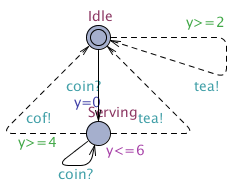
\includegraphics[scale=0.7]{images/bev_machine_model}
\par\end{centering}
\caption{Model of beverage-serving machine.}
\label{bev-machine}
\end{figure}

The preceding figure (see fig. \ref{bev-machine}) illustrates the model of beverage-serving machine. Given a coin (\emph{coin}), it serves either coffee (\emph{cof}) 
or tea (\emph{tea}) within a given time interval. Moreover, free tea is served once in a while. In the example, the TIOA consists of and two locations represented by 
circles: \emph{Idle} and \emph{Serving}. \emph{Idle} represents the starting location, and the state of machine waiting for coin input (\emph{coin?}).  
 The flow of TIOA is controlled by three types of labels: \emph{invariants}, \emph{guards} and \emph{clock-reset operations}. 
Invariants are defined on locations ($y\leq 6$) and represent constraints for the clocks in order for the control to remain in particular location until time requirement is fulfilled.  
Guards are located on the edges ($y\geq 2$ and $y\geq 4$) and express conditions on the values of clock that must be satisfied in order for 
the edge to be taken. When the condition is satisfied, the transition occurs and action (\emph{cof!} or \emph{tea!}) is triggered. Clock-reset operations ($y=0$) are simple
clock value manipulations in form of assignment that enforce progress in the system.

In ECDAR, the specification interface is leveraging the UPPAAL TIGA language \cite{behrmann_uppaal-tiga:_2006} to describe TIOA. However, the following constraints are retained\footnote{See \href{http://people.cs.aau.dk/adavid/ecdar/examples.html\#lang}}:   
%
\begin{itemize}
\item Invariants may not be strict.
\item Inputs must use controllable edges.
\item Outputs must use uncontrollable edges.
\item All channels must be declared broadcast.
\item The system is implicitly input enabled due to broadcast communication but for refinement checking purposes the relevant inputs must be explicit in the model.
\item In the case of parallel composition of several components, a given output must be exclusive to one component.
\item For implementations, outputs must be urgent.
\item For implementations, every state must have independent time progress, i.e., progress must be ensured by either an output or infinite delay.
\item $\tau$-transitions (no output or input) are forbidden. %There was a comment about this item%
\item Global variables are forbidden.
\end{itemize}

\subsection{Code Generation \label{background-codegeneration}}
In order to clarify what code generation is one need to understand what a model transformation is, as this is a fundamental part of code generation. In short one could say that the model transformation is a way to ensure that the final code is consistent and with a reduced number of errors. The generation is an automated way to produce code from models. The actual generation is defined by the software developer, thus it is defined what the output should be, but the input and the data is not.

There is generally two ways to do model transformations, that is model to model and model to text, the former known as M2M and the latter M2T. There are also a lot of other tools and techniques for transformation, which should not be confused with model transformations. One could mention an XSLT-transformation as an example, where the base input is an XML-document and the final output is another XML-document, often XHTML, with a predefined XML-Schema.

Model to model is a transformation of a number of models to a given number of new models - from X number of models to Z number of new models. Model to text is the transformation of a number of models to text, the text could for instance be code - which is why the process sometimes is known as model to code.


